\RequirePackage{plautopatch}
\documentclass[uplatex,dvipdfmx,a4paper,10pt]{jsarticle} %!
\usepackage{graphicx} %!
\usepackage{amsmath} %!
% \usepackage{float}
\usepackage{csvsimple}
\usepackage{url}

\title{放射線の計測}
\author{電気通信大学 I\hspace{-1.2pt}I\hspace{-1.2pt}I類\\
2313213 山口海音} %!!!
\date{\today 作成} %!!!

\begin{document}
\maketitle
\section{目的} %!
第1に，我々が普段どれほどの放射線を被っているかを知る．第2に，自然界に存在する放射性原子を調べる．第3に，放射性原子からの放射線を測定することで，崩壊の時間的ランダム性と，放射の等方向性を確かめる．第4に，放射線をある物質に吸収させることで，その物質の質量吸収係数を求め，放射線の遮蔽に適した物質について考える．
\section{原理}
\subsection{放射性原子の崩壊}
放射性原子とは，その原子核の不安定さのために，より安定な原子核へ変化する性質を持つ原子である．また，この変化を崩壊といい，この際に原子核の外へ放射されたものを放射線という．放射線にはアルファ線（中性子2個，陽子2個からなる原子核），ベータ線（電子），ガンマ線（電磁波）がある．

放射は一定の確率で起こることが知られている．このため，単位時間当たりの放射回数はポアソン分布に従う．

放射は全方位に等しい確率で起こることが知られている．これは，図\ref{invsqrt}のように中心から放射する矢印の数として考えると分かり良い．
\begin{figure}[htbp]
    \begin{center}
    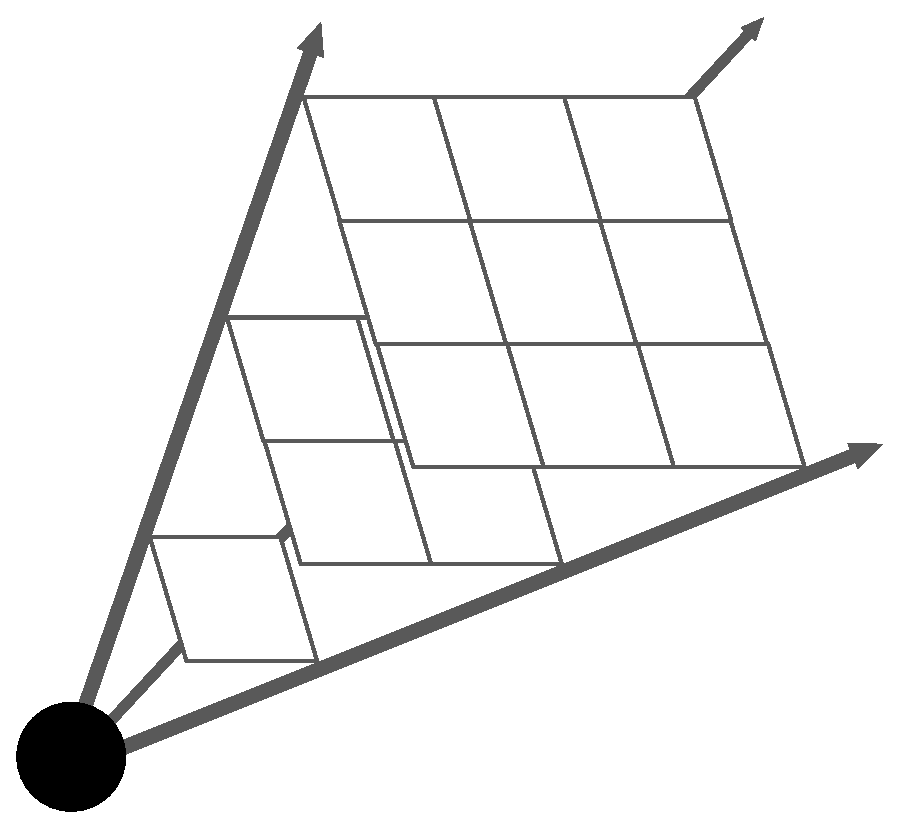
\includegraphics[scale=0.3]{material/islaw.eps}
    % \includesvg{material/xprmtFig.svg}
    \caption{逆二乗則の考え方}
    \label{invsqrt}
    \end{center}
\end{figure}
このため，単位面積，単位時間当たりの放射回数は逆二乗則に従う．即ち，一定の面積に対する計数値$N$と放射線源との距離$r$の間に以下の関係が成り立つ．
\begin{equation}
    N \propto \frac{1}{r^2}
\end{equation}

セシウムは放射性原子の一種である．崩壊によって以下のような反応を起こす．
\begin{equation}
    {}^{137}_{55}\mathrm{Cs} \rightarrow {}^{137}_{56}\mathrm{Ba} + \mathrm{e}^{-} + \bar{\nu}_e 
\end{equation}
\subsection{GM計数管}
ガイガー・ミューラー計数管は，図\ref{gm_meter} に示すような放射の検出器である．その円筒状の陰極から直線状の陽極までには，$500$ - $1000\mathrm{V}$の電位差があり，円筒内部にはアルゴンガスとアルコールなどが封入されている．これにより放射線が入ってきたときに放電が起こるのでこれを計測することで放射が検出できる．
\begin{figure}[htbp]
    \begin{center}
    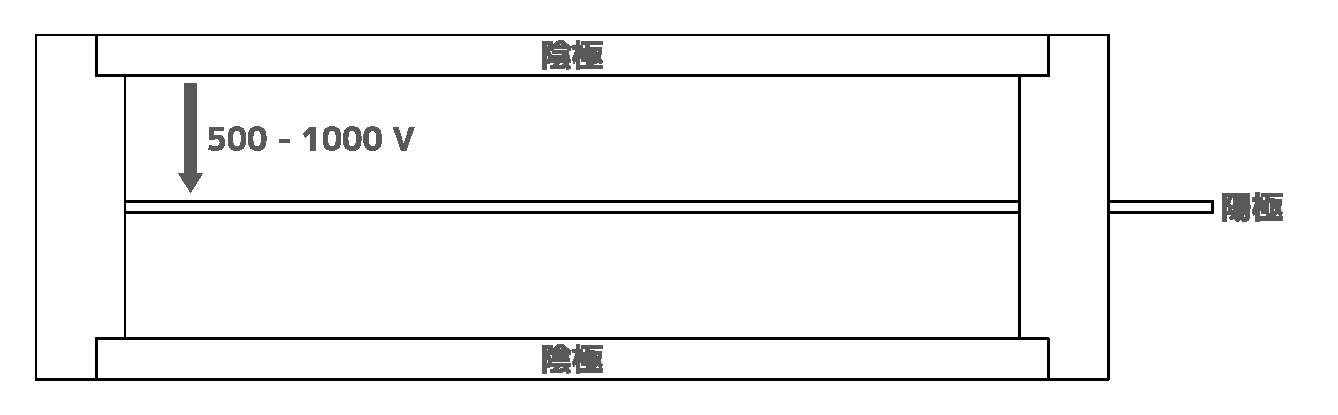
\includegraphics[scale=0.6]{material/gm_meter.eps}
    % \includesvg{material/xprmtFig.svg}
    \caption{ガイガー・ミューラー計数管}
    \label{gm_meter}
    \end{center}
\end{figure}
\subsection{β線の吸収}
ベータ線が物質中を通過するとき，一部がその物質との相互作用によりエネルギーを失って物質中に残ってしまう．特に，ある極めて薄い厚さの物質中を通過することによって失われる物質の個数$-\Delta N$は，元の個数$N$に比例し，その比例定数は$N$に依らず一定であることが知られている．即ち，以下が成立する．
\begin{equation}
    -\Delta N \propto N
\end{equation}
そのため，このときの厚さの$\Delta x$倍の物質を通過するときには$-\Delta N \propto N\Delta x$だけ物質の個数が小さくなる．この比例定数を線吸収計数$\mu$とする．これはその物質がどれだけ放射線の遮蔽にすぎれているかを示す．また，この値をその物質の密度で割ることで，密度あたりの遮蔽性能を表す質量吸収計数$\mu_\mathrm{m}$が得られる．

\section{実験方法}
図\ref{xprmt_fig}に示すような実験装置を用いて放射線を計測する．まず，電源スイッチをオンにする．次に，印加電圧調整つまみを操作して電圧指示計が$500\mathrm{V}$を示すように調整する．この後の実験はこの電圧を保ったまま行われる．
\begin{figure}[htbp]
    \begin{center}
    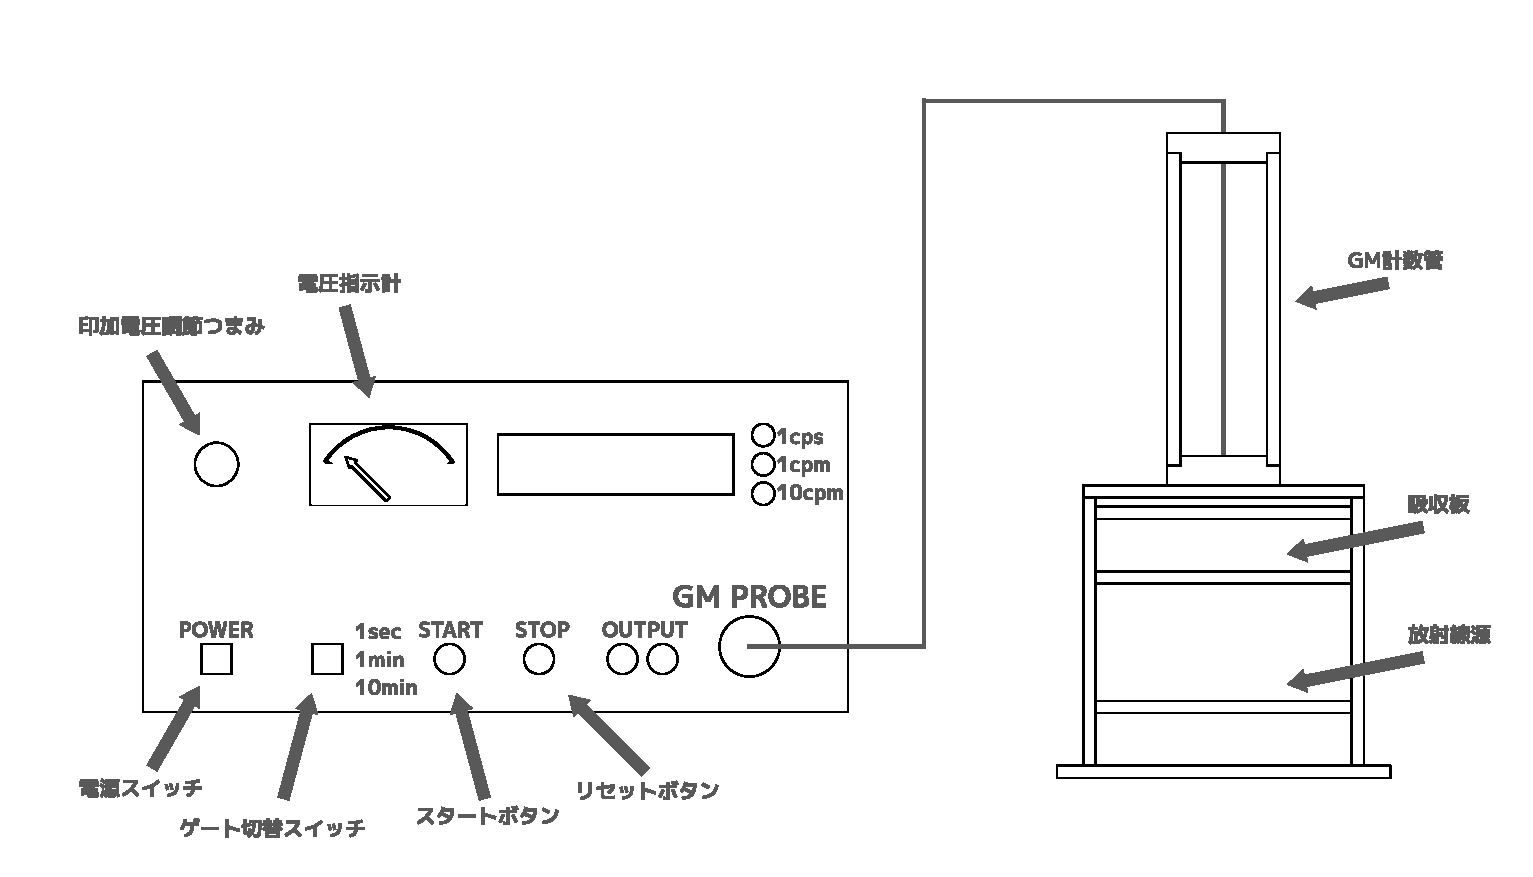
\includegraphics[scale=0.6]{material/xprmtFig.eps}
    % \includesvg{material/xprmtFig.svg}
    \caption{実験装置の概略図}
    \label{xprmt_fig}
    \end{center}
\end{figure}
\subsection{自然計数の計測}
まず，ゲート切替スイッチを`$1$min'にする．このとき計数切替表示ランプが`cpm'になっていることを確認する．次に，リセットボタンを押し，スタートボタンを押し，$1$分待って，計数値を記録する，という操作を$20$回繰り返す．

\subsection{放射線源の距離に依る計数の測定}
まず，放射線源を距離$60$の位置に置く．次に，ゲート切替スイッチを`$1$sec'にする．次に$400$回測定する．放射線源の距離を$30$, $120$に変えて同様に実験する．

\subsection{吸収板に依る$\beta$線の吸収の測定}
まず，放射線源を距離$60$の位置に置く．次に，ゲート切替スイッチを`$1$min'にする．次に，$4$回測定し，$1$枚吸収板を距離$30$の位置に置く，という操作を，事前に用意した吸収板がなくなるまで繰り返す．これを，Al板$1$枚，Ti板$5$枚，Ni板$6$枚の場合でそれぞれ行う．
\section{実験結果}
\subsection{自然計数の計測}
自然計数の計測結果を図\ref{NCrslt}に示す．また，自然計数の平均$\langle N\rangle$は$15.4\mathrm{cpm}$であった．
\begin{figure}[ht]
    \begin{center}
    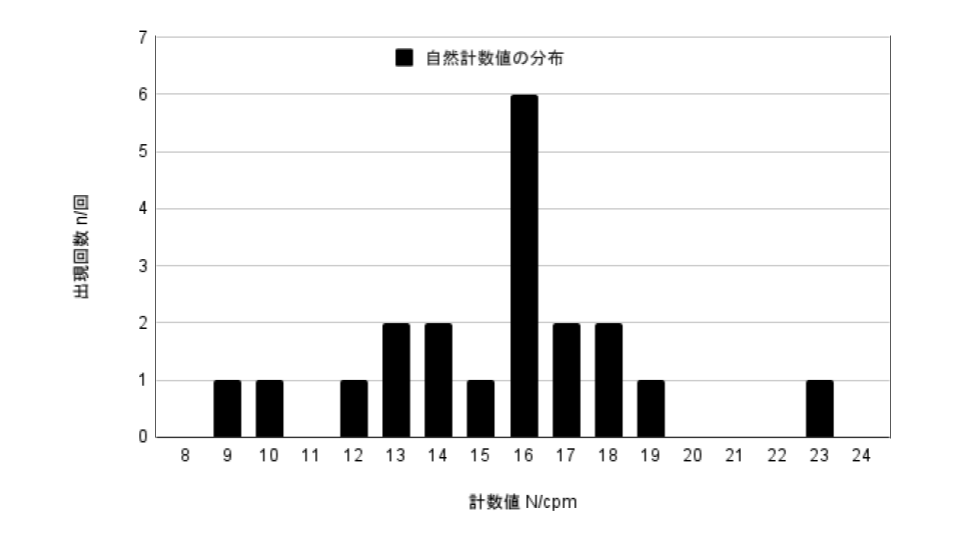
\includegraphics[scale=0.3]{material/NCrslt.png}
    \caption{自然計数の計測結果}
    \label{NCrslt}
    \end{center}
\end{figure}

\subsection{放射線源の距離に依る計数の測定}
放射線源とGM計数管の距離を$30\mathrm{mm}$，$60\mathrm{mm}$，$120\mathrm{mm}$と変えて$100$回計測したのち，$300$回計測した．このときの計数値ごとの出現回数の割合を図\ref{d30t100}，\ref{d30t300}，\ref{d60t100}，\ref{d60t300}，\ref{d120t100}，\ref{d120t300}に示す．
\begin{figure}[ht]
    \begin{center}
    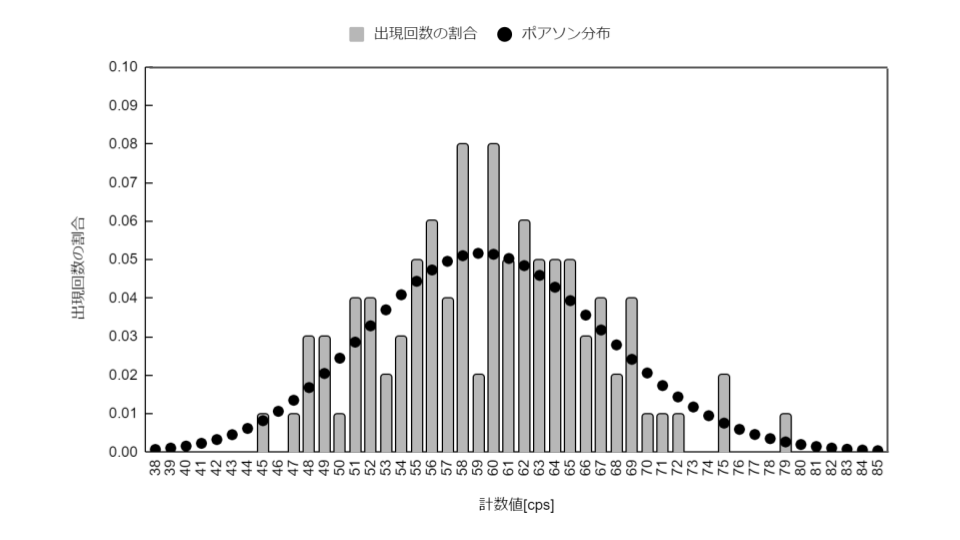
\includegraphics[scale=0.3]{material/d30t100.png}
    \caption{距離30，計測回数100}
    \label{d30t100}
    \end{center}
\end{figure}
\begin{figure}[ht]
    \begin{center}
    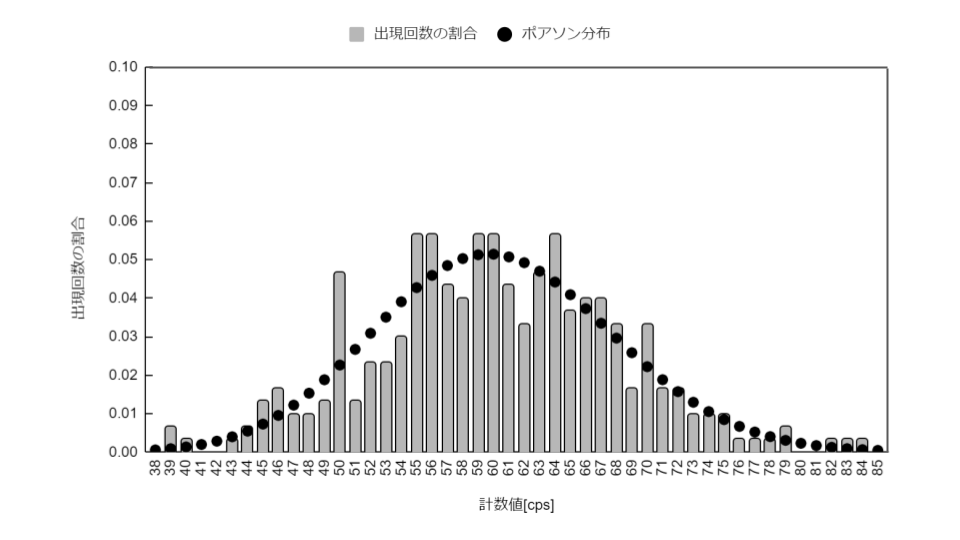
\includegraphics[scale=0.3]{material/d30t300.png}
    \caption{距離30，計測回数300}
    \label{d30t300}
    \end{center}
\end{figure}
\begin{figure}[ht]
    \begin{center}
    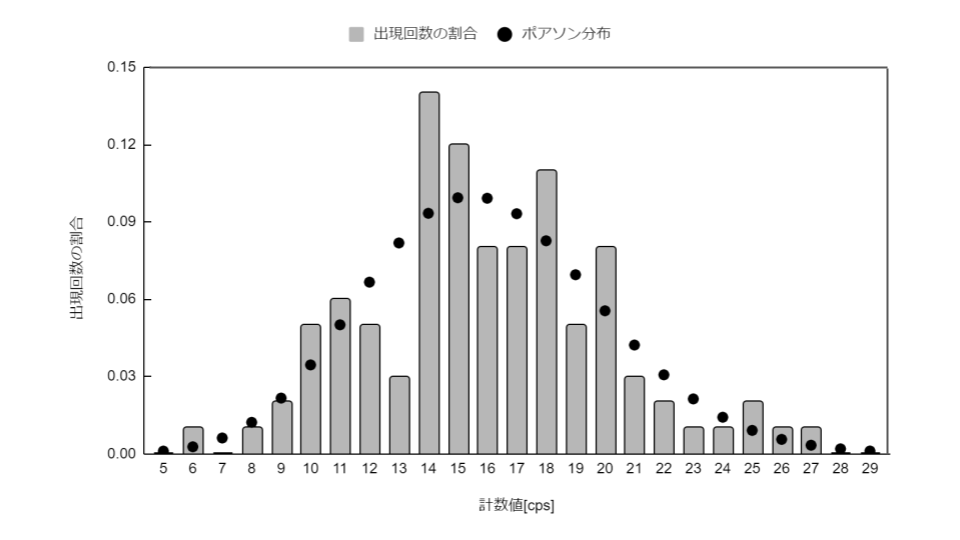
\includegraphics[scale=0.3]{material/d60t100.png}
    \caption{距離60，計測回数100}
    \label{d60t100}
    \end{center}
\end{figure}
\begin{figure}[ht]
    \begin{center}
    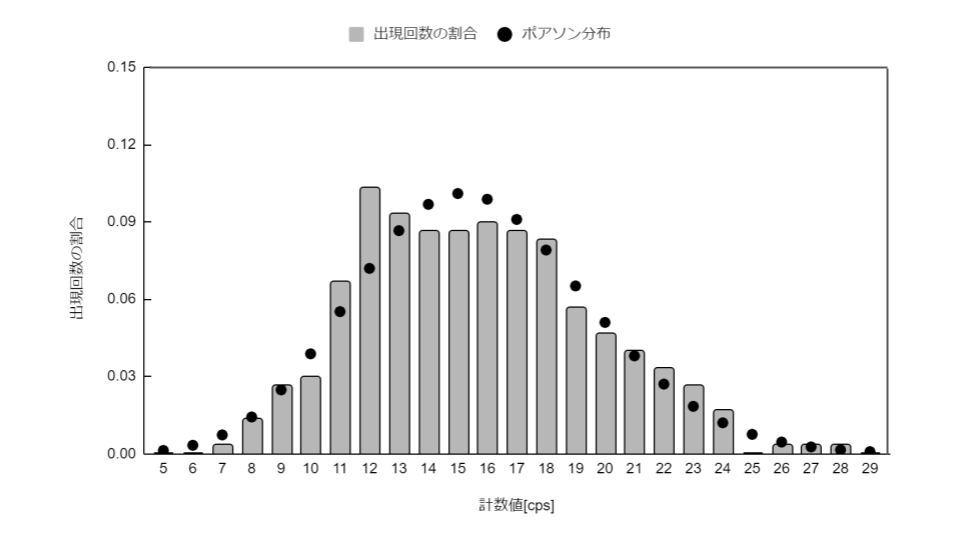
\includegraphics[scale=0.3]{material/d60t300.png}
    \caption{距離60，計測回数300}
    \label{d60t300}
    \end{center}
\end{figure}
\begin{figure}[ht]
    \begin{center}
    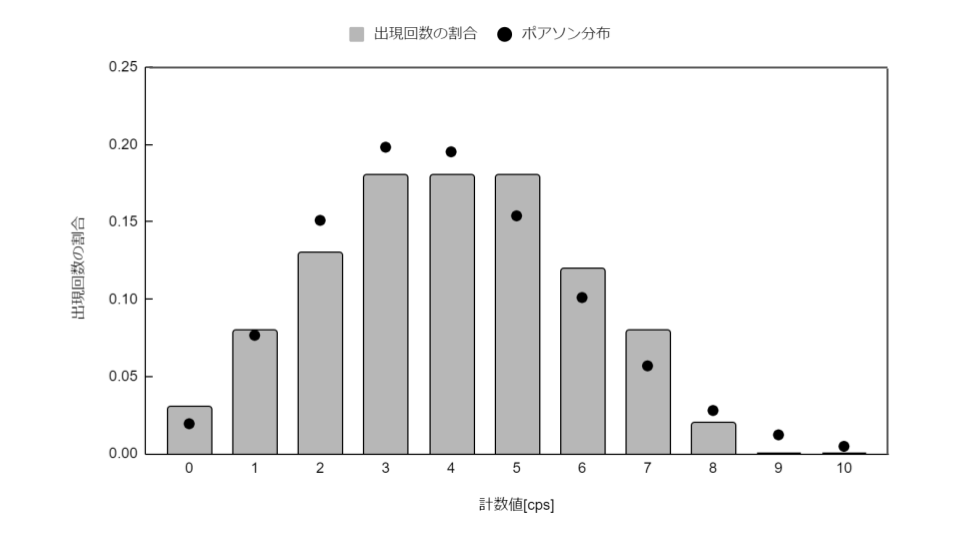
\includegraphics[scale=0.3]{material/d120t100.png}
    \caption{距離120，計測回数100}
    \label{d120t100}
    \end{center}
\end{figure}
\begin{figure}[ht]
    \begin{center}
    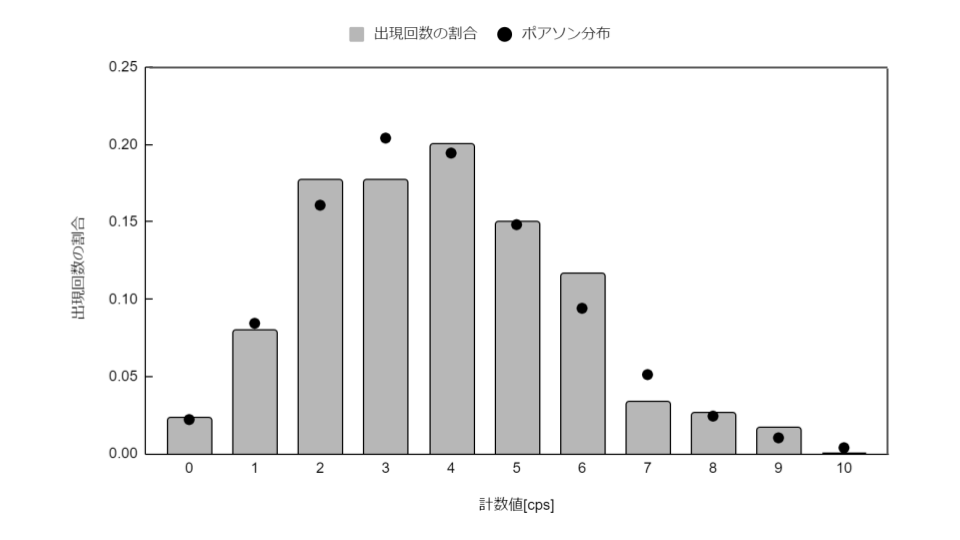
\includegraphics[scale=0.3]{material/d120t300.png}
    \caption{距離120，計測回数300}
    \label{d120t300}
    \end{center}
\end{figure}

\subsection{吸収板に依る$\beta$線の吸収の測定}
Ti板とNi板に依る$\beta$線の吸収の実験データをそれぞれ表\ref{tidata}，\ref{nidata}に示す．
\begin{table}
    \caption[Tiの$\beta$線の吸収の実験データ]{Tiの$\beta$線の吸収の実験データ}
    \label{tidata}
    \begin{center}
    \begin{tabular}{l|lrrrrrrr}
        \hline
        枚数 & 厚さ$x/\mathrm{mm}$ & $1$分間の計数値$N/\mathrm{cpm}$ & 平均値$\langle N\rangle/\mathrm{cpm}$ & $\beta$線計数値$\langle N_\mathrm{\beta}\rangle/\mathrm{cpm}$ & 対数$log_{10}{\langle N_\mathrm{\beta}\rangle}$ & 標準偏差$/\mathrm{cpm}$ & $log_{10}{\left(\langle N_\mathrm{\beta}\rangle -\sigma_\mathrm{\beta}\right)}$ & $log_{10}{\left(\langle N_\mathrm{\beta}\rangle + \sigma_\mathrm{\beta}\right)}$\\ \hline
        \csvreader[late after line=\\]{material/tidata.csv}
        {num=\num, thi=\thi, one=\one, mea=\mea, bet=\bet, log=\log, std=\std, lnl=\lnl, lnu=\lnu}
        {\num&\thi&\one&\mea&\bet&\log&\std&\lnl&\lnu}
        \hline
    \end{tabular}
    \end{center}
\end{table}

\begin{table}
    \caption[Niの$\beta$線の吸収の実験データ]{Niの$\beta$線の吸収の実験データ}
    \label{nidata}
    \begin{center}
    \begin{tabular}{l|lrrrrrrr}
        \hline
        枚数 & 厚さ\\$x/\mathrm{mm}$ & $1$分間の計数値$N/\mathrm{cpm}$ & 平均値$\langle N\rangle/\mathrm{cpm}$ & $\beta$線計数値$\langle N_\mathrm{\beta}\rangle/\mathrm{cpm}$ & 対数$log_{10}{\langle N_\mathrm{\beta}\rangle}$ & 標準偏差$/\mathrm{cpm}$ & $log_{10}{\left(\langle N_\mathrm{\beta}\rangle -\sigma_\mathrm{\beta}\right)}$ & $log_{10}{\left(\langle N_\mathrm{\beta}\rangle + \sigma_\mathrm{\beta}\right)}$\\ \hline
        \csvreader[late after line=\\]{material/nidata.csv}
        {num=\num, thi=\thi, one=\one, mea=\mea, bet=\bet, log=\log, std=\std, lnl=\lnl, lnu=\lnu}
        {\num&\thi&\one&\mea&\bet&\log&\std&\lnl&\lnu}
        \hline
    \end{tabular}
    \end{center}
\end{table}

\section{調査結果}
\subsection{自然界に存在する放射性原子とその放射線の種類，半減期}
表\ref*{radatom}に放射性原子とその放射線の種類，半減期について調べた結果を示す（\cite{qanda}p. 273.）．
\begin{table}
    \caption[放射性原子]{放射性原子とその放射線，半減期}
    \label{radatom}
    \begin{center}
    \begin{tabular}{l|lr}
        \hline
        放射性原子の核 & 放射線 & 半減期[年] \\ \hline
        \csvreader[late after line=\\]{material/radiation_nuclear.csv}
        {element=\ele, mass=\mass, radline=\line, halflife=\half}
        {${}^{\mass}\mathrm{\ele}$ & \line & \half}
        \hline
    \end{tabular}
    \end{center}
\end{table}
\section{考察}
% \subsection{普段浴びている放射線}
\subsection{自然界の放射線}
調査の結果自然界には様々な放射性原子による放射が起きていると分かった．
\subsection{崩壊の時間的ランダム性}
放射線源の距離に依る計数の測定の図において，確かにポアソン分布に従ていると考えられるので原子の崩壊は時間的にランダム即ち，ある時間間隔における崩壊確率は一定であると分かる．
% \subsection{放射の等方向性}
% \subsection{放射線を吸収しやすい物質}
\begin{thebibliography}{99}
    \bibitem{qanda} 大塚徳勝・西谷源展，『Q\&A 放射線物理』改訂新版，2007年，共立出版株式会社．
    \bibitem{measure} 河田燕，『放射線計測技術』初版，1978年，東京大学出版会．
    \bibitem{sciyear} 理科年表プレミアム，理科年表オフィシャルサイト，国立天文台・丸善出版，2023-06-23閲覧，\url{https://www.rikanenpyo.jp/member/?module=Member&p=Contents%26page%3DMS1catD%3AD%5EContents%26page%3D1_cPSx11x0150_2023_1%3Aco&action=Contents&page=1_cPSx11x0150_2023_1}.
\end{thebibliography}

\end{document}